\documentclass[a4paper,10pt]{article}
\usepackage{caption}
\usepackage[utf8x]{inputenc}
\usepackage{graphicx}
\usepackage[hmargin=3cm,vmargin=3cm]{geometry}
%opening
\title{}
\author{}

\begin{document}

% \maketitle

% \begin{abstract}

% \end{abstract}

% \section{Prelimniary results, frist step}
% cf. master thesis simon Carrignon
% 
% \section{How to handle the lazarus effect}
% 
% Add a maturation mechanism :
% 
% When an agent die because he don't find any energy, he is refilled when he receveid a new genome after a certain wainting time. The maturation effect says that when the robot will move again he will not be able to share its genome till he have not get energy from the environment
% 
% \section{Tests of different kind of environments }
%  Here are stored differents kind of environment tested for differents reasons
% \subsection{Test random suns in two opposit sides vs a first 8-like environment}
% \subsubsection{pressure on generalist to little (Bad foraging reward function BFRF)}
%  
% 
% {\tiny
% \begin{verbatim}
% 
% ConfigurationLoaderObjectName=MedeaSpConfigurationLoader
% VisibleEnergyPoint=true
% VisibleLockedEnergyPoint=true
% gB=0
% gBackgroundImageFilename=data/simple_zones.png
% gBatchMode=true
% gDeadTime=1.5
% gDeltaKey=2.0
% gDenPen=false
% gDisplayMode=1
% gDisplaySensors=false
% gDisplayZoneCaption=false
% gDriftEvaluationRate=1.0
% gDriftLock=2.0
% gDynaStep=0.35
% gDynamicRespawn=true
% gDynamicSigma=true
% gEnergyInit=1800
% gEnergyMax=800
% gEnergyMode=true
% gEnergyPointRadius=40.0
% gEnergyPointRespawnLagMaxValue=0
% gEnergyPointValue=200
% gEnergyRevive=200
% gEnvironmentImageFilename=data/simple_environment.png
% gEvaluationTime=800
% gExperiment1_genStart=1000000
% gExperiment2_genStart=10000000
% gExperimentNumber=1
% gFastDisplayModeSpeed=60
% gForegroundImageFilename=data/simple_environment.png
% gMaxEnergyPoints=2
% gMaxIt=400000
% gN=20
% gNbOfAgents=100
% gNbTypeResource=2
% gRandSun=false
% nbHiddenNeurons=5
% nbLayer=1
% \end{verbatim}
% }


% Bad reward function :
% \begin{figure}[h]
% 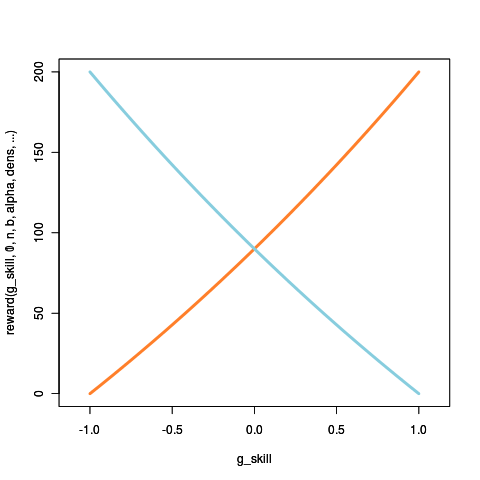
\includegraphics[height=4cm]{images/generalFitness.png} 
% \caption{this kind of foraging function allow generalist}
% \end{figure}
% 
% In this environment pressur on generalist is too faible. Allow us to look at the new 8-like environment, and see that he is able to maintain generalists.
% 
% \paragraph{Alea opposit sides}
% See fig.\ref{aleaOSBFRF}
% \begin{figure}
% \centering
% \caption{{\huge Alea opposit sides with exp function}(200runs)}
%  \label{aleaOSBFRF}
%  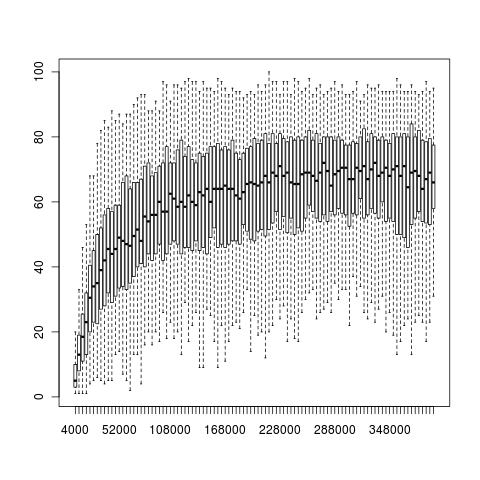
\includegraphics[height=4cm	]{images/aleaAliveBFRF.png}
%  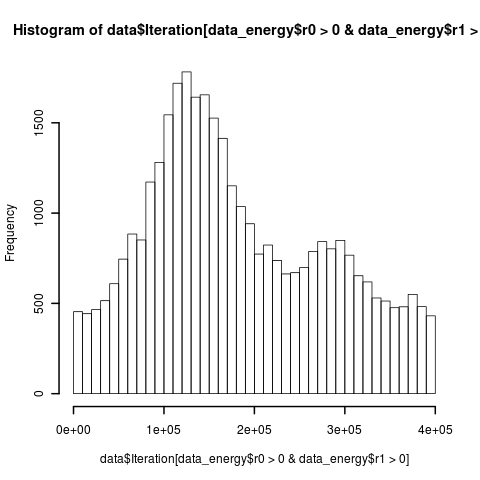
\includegraphics[height=4cm	]{images/aleaHistEnergBFRF.png}
%  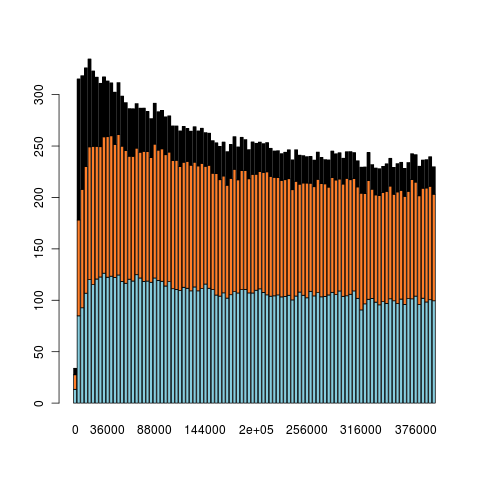
\includegraphics[height=6cm	]{images/aleaBarPlotEnergyBFRF.png}
% \end{figure}
% 
% 

% \paragraph{8-like}
% 
% A full circle of the 8 (cf. \ref{fig:8-like}) is done after 20 sun movments ; a movments is done each 1000 iteration, so a full circle is made after 20000 iteration. 
% 
% \begin{figure}[H]
% \caption{Allowed positions of energy points during simulation (numbers are just id, not an order)}
% \label{fig:8-like}
% \centering
% 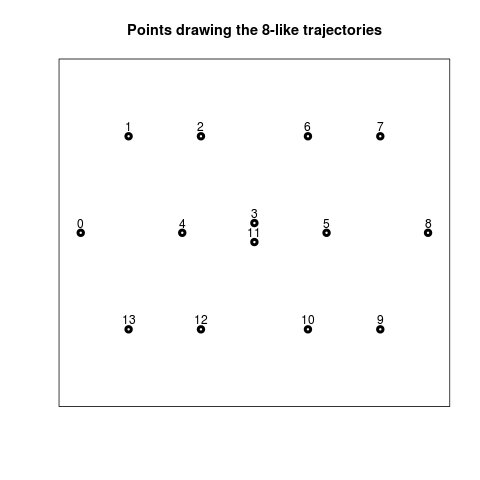
\includegraphics[width=.5\textwidth]{images/traj8like}
% \end{figure}
% % 
% See fig.\ref{trajOSBFRF}
% \begin{figure}
%  \label{trajOSBFRF}
% \centering
% \caption{{\huge 8-like with exp function} (200runs)}
%  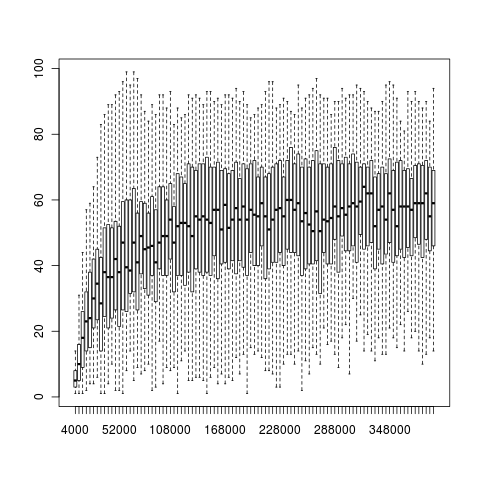
\includegraphics[height=4cm	]{images/trajAliveBFRF.png}
%  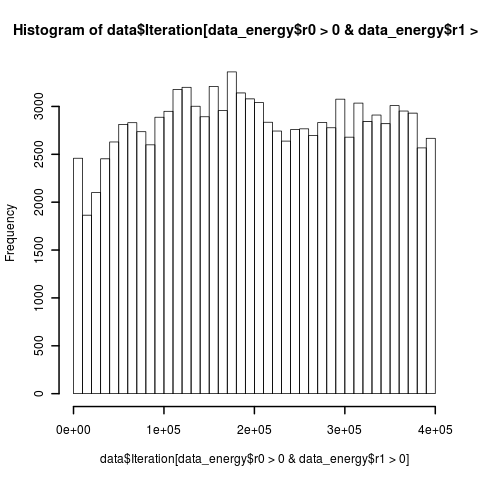
\includegraphics[height=4cm	]{images/trajHistEnergBFRF.png}
%  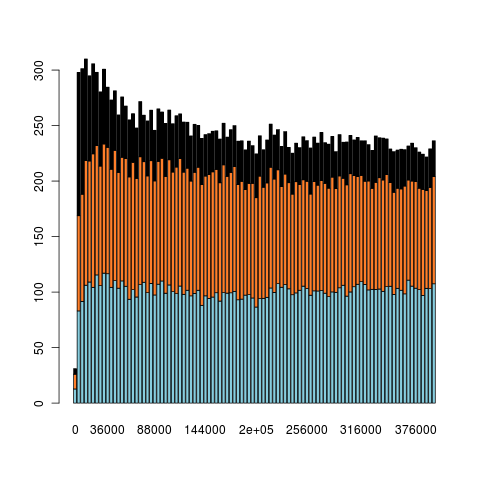
\includegraphics[height=6cm	]{images/trajBarPlotEnergyBFRF.png}
% \end{figure}
% 
% 
% \paragraph{Analyse}
% 
% Medea solves the two environments in similar way : \textbf{$43.29268\%$} of the run in the first environment go to 400000 iterations, VS \textbf{$42.94872\%$} in the second one ; and also the number of alive in both environments is almost similare (no stat,). 
% 
% Without any surprise the only difference is that the 8-like environment allows generalists to survive, because suns meet themsleves thrice all 5 suns change (one sun change all 1000 iteration, so all 5000 iterations). 
% \subsubsection{Tanh Shaped reward function}
% \begin{figure}[h]
% \centering
% 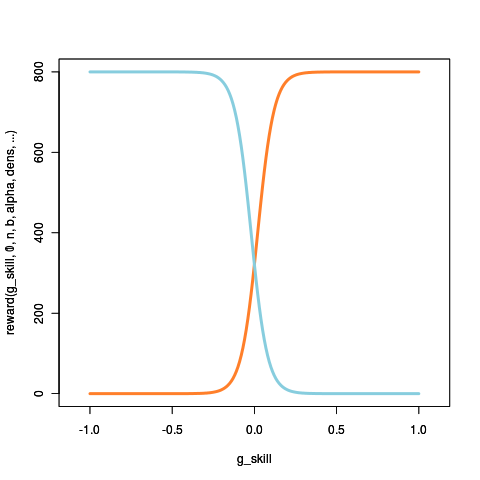
\includegraphics[height=4cm]{images/TanhShaped.png} 
% % \caption{this kind of foraging function allow generalist}
% \end{figure}
% 
% \paragraph{Random}
% \begin{figure}
% \label{aleaTanh}
% \centering
% \caption{{\huge Rand Sun with Tanh function}(400runs))}
% 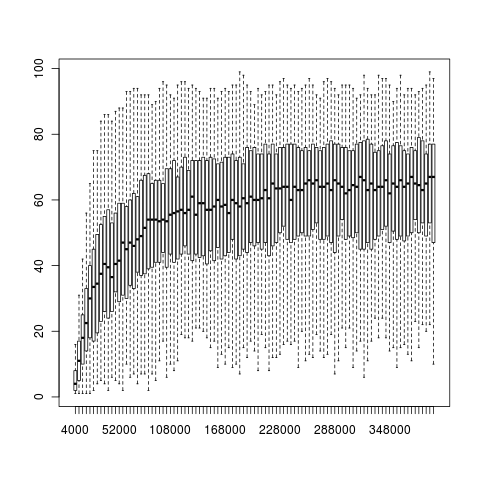
\includegraphics[height=4cm]{images/aleaTanhAlive.png}
% 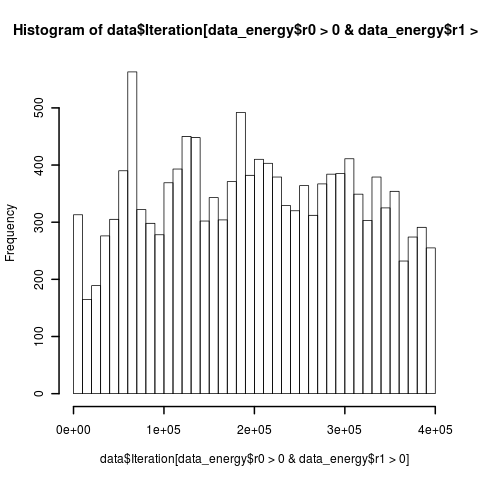
\includegraphics[height=4cm]{images/aleaTanhHistEnerg.png}
% 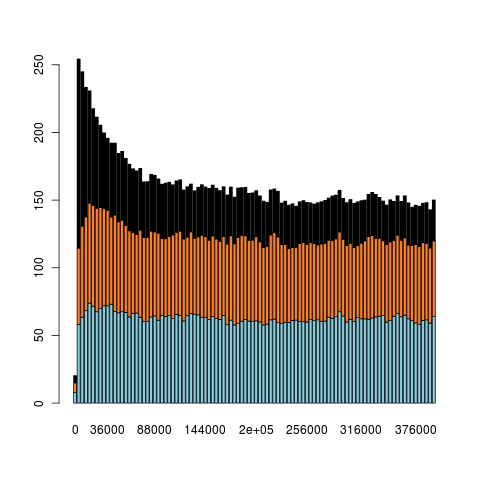
\includegraphics[height=6cm]{images/aleaTanhBarPlotEnergy.png}
% \end{figure}
% 
% \paragraph{8-like}
% \begin{figure}
% \label{trajTanh}
% \centering
%  \caption{ {\huge 8-like with Tanh function} (200runs)}
% 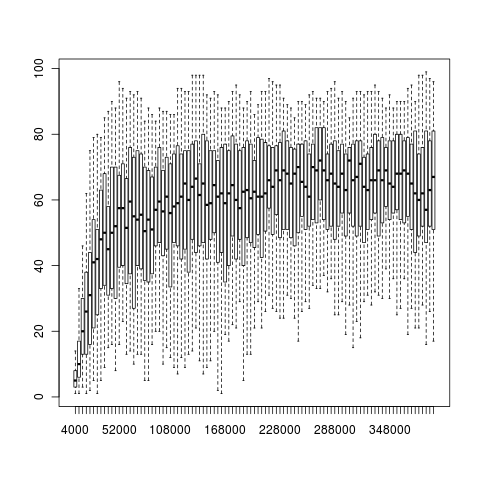
\includegraphics[height=4cm]{images/trajTanhAlive.png}
% 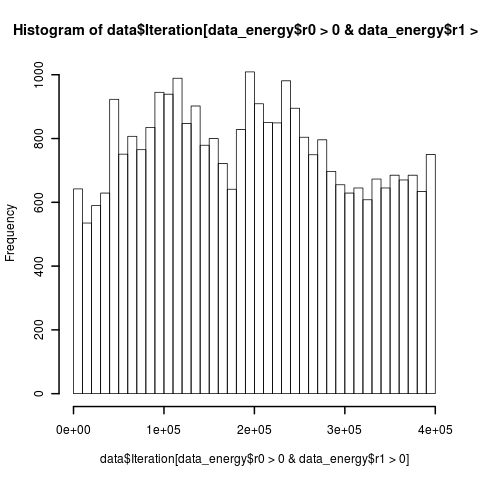
\includegraphics[height=4cm]{images/trajTanhHistEnerg.png}
% 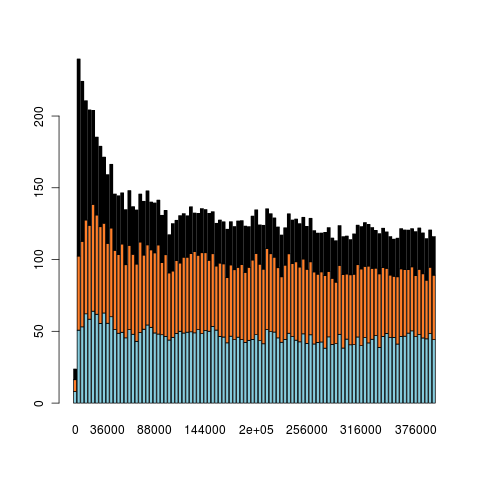
\includegraphics[height=6cm]{images/trajTanhBarPlotEnergy.png}
% \end{figure}
% 
% \paragraph{Analyse}
% 
% This time environment is harder to solve : $32,5\%$ in 8like (over 200runs), $28,5\%$ in random (over 406runs) of runs continu during 400000 iterations. As expected we don't find the différence beetwen the number of generalists, as the pressure toward them iss really high.
% 
% \section{Test avec maturation, et surtout periode de preparation}
% 
% \paragraph{E:8l;r:t;lr;mt}
% \begin{figure}
% \label{env-8l_rew-t_res-l_math}
% \centering
% \caption{ {\huge env-8l\_rew-t\_res-l\_math} (200runs)}
% 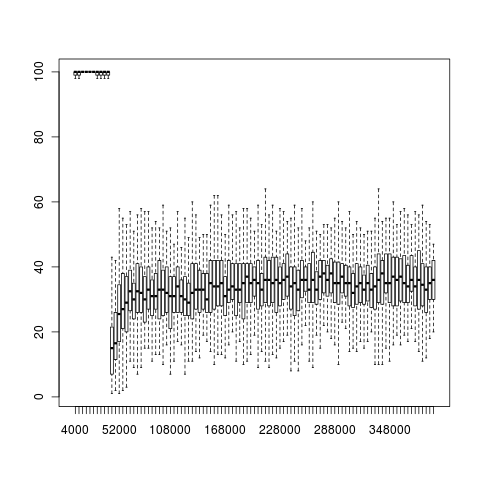
\includegraphics[height=4cm]{images/env-8l_rew-t_res-l_mathAlive.png}
% 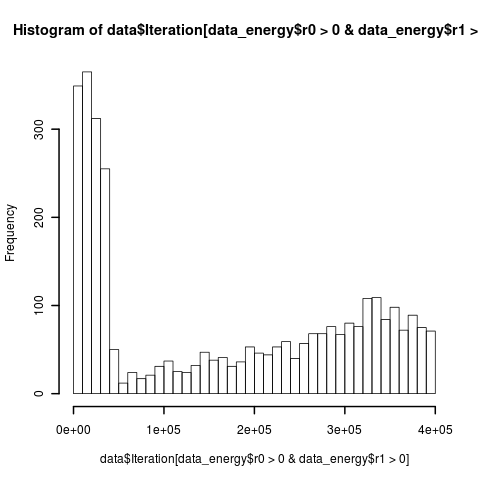
\includegraphics[height=4cm]{images/env-8l_rew-t_res-l_mathHistEnerg.png}
% 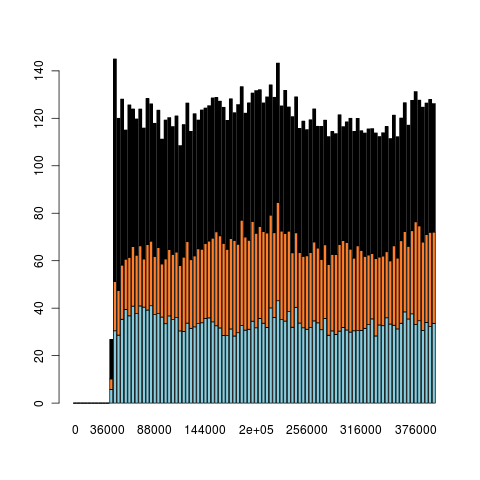
\includegraphics[height=6cm]{images/env-8l_rew-t_res-l_mathBarPlotEnergy.png}
% \end{figure}
% 
% \paragraph{E:8l;r:t;nlr;mt TMax = 1million iterations}
% \begin{figure}
% \label{env-8l_rew-t_res-nl_mat_tmax-1Mh}
% \centering
% \caption{ {\huge env-8l\_rew-t\_res-nl\_math} (200runs,Max = 1million iterations)}
% 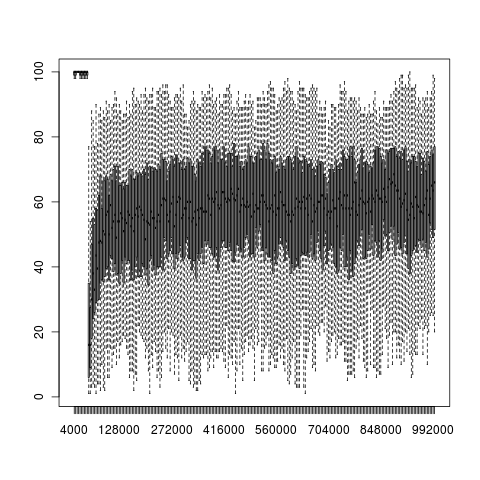
\includegraphics[height=4cm]{images/env-8l_rew-t_res-nl_mat_tax-1MhAlive.png}
% 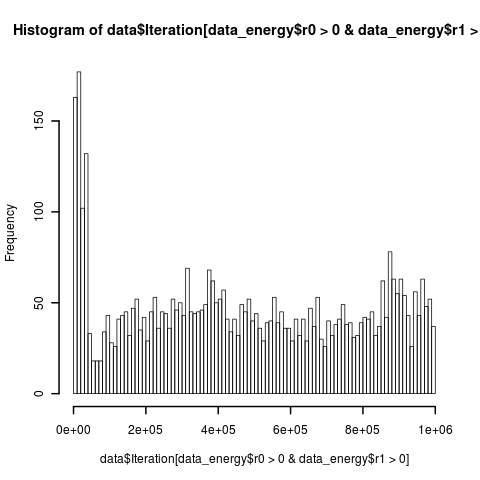
\includegraphics[height=4cm]{images/env-8l_rew-t_res-nl_mat_tax-1MhHistEnerg.png}
% 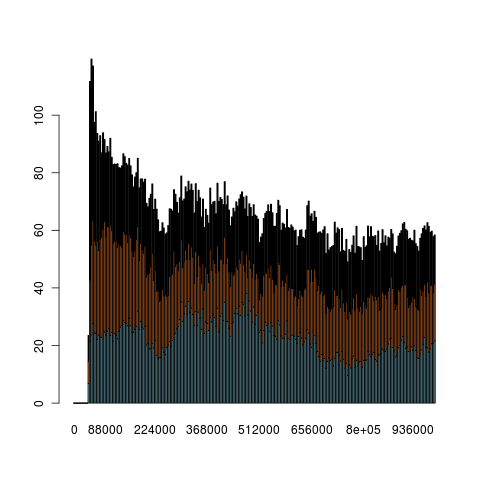
\includegraphics[height=6cm]{images/env-8l_rew-t_res-nl_mat_tax-1MhBarPlotEnergy.png}
% \end{figure}
% 
% \paragraph{E:8l;r:t;lr;mt TMax = 1million iterations}
% \begin{figure}
% \label{env-8l_rew-t_res-l_mat_tmax-1Mh}
% \centering
% \caption{ {\huge env-8l\_rew-t\_res-l\_math} (200runs,Max = 1million iterations)}
% 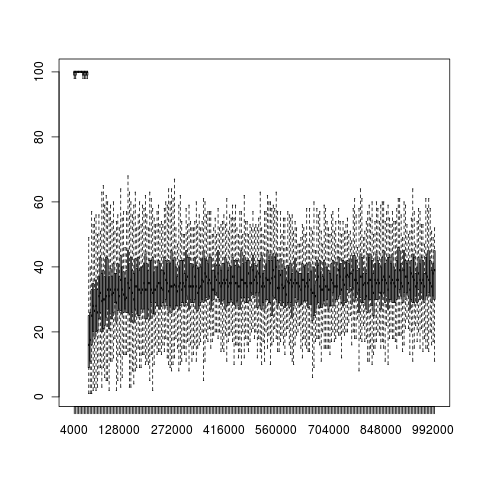
\includegraphics[height=4cm]{images/8likeEnv/env-8l_rew-t_res-l_mat_tax-1MhAlive.png}
% 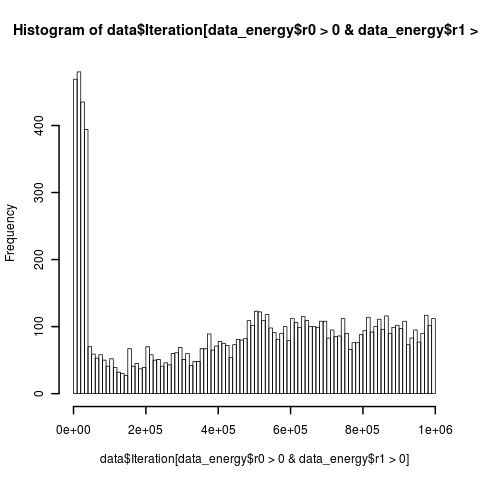
\includegraphics[height=4cm]{images/8likeEnv/env-8l_rew-t_res-l_mat_tax-1MhHistEnerg.png}
% \end{figure}
% 
% % \inclte ressources}
% In order to limit ressource, differents strategies tested :
% \begin{itemize}
% \item ressource have limited energy capacities: $Q_E$
% \item $Q_E=\#Robot_{allowed} * argmin(1,\frac{\#Robot_{allowed}}{\#Robot_{t-n}})$ le second terme permet d'ajouter une "memoire" au fruit pour eviter syncronisation..
% \item The amount of energy foraged : $q_e= \alpha>=1$ 
% \begin{itemize}
% \item if $q_e==1$ : robots can stay alive on the source,
% \item else allow robots to survive longer, should be $\alpha >= d_{sun}$ in order to alloew robots to follow the soruce at its next place
% \end{itemize}
% \begin{figure}
% \label{trajTanh}
% \centering
% \caption{ {\huge 8-like with Tanh function With limited ressources} (runs)}
% 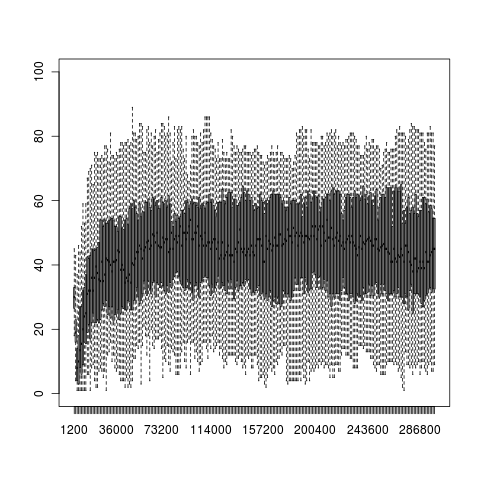
\includegraphics[height=4cm]{images/8likeEnv/alive_8like_pressure50}
% % \includegraphics[height=4cm]{images/8likeEnv/trajLimitedTanhHistEnerg.png}
% % \includegraphics[height=6cm]{images/8likeEnv/trajLimitedTanhBarPlotEnergy.png}
% \end{figure}
% \end{itemize}
% udegraphics[height=6cm]{images/env-8l_rew-t_res-l_mat_tax-1MhBarPlotEnergy.png}
% \end{figure}


% \paragraph{E:8l;r:t;nlr;mt}
% \begin{figure}
% \label{env-8l_rew-t_res-nl_math}
% \centering
% \caption{ {\huge env-8l\_rew-t\_res-nl\_math} (200runs)}
% 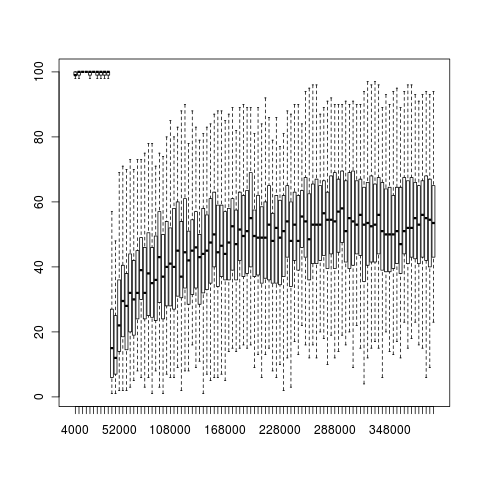
\includegraphics[height=4cm]{images/env-8l_rew-t_res-nl_mathAlive.png}
% 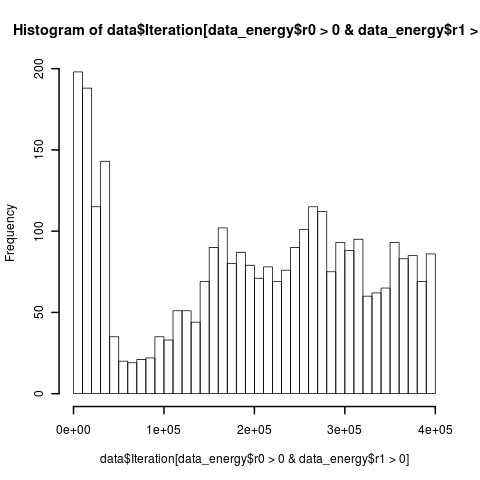
\includegraphics[height=4cm]{images/env-8l_rew-t_res-nl_mathHistEnerg.png}
% 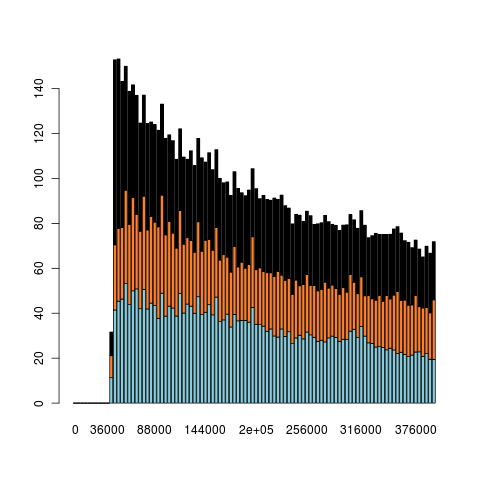
\includegraphics[height=6cm]{images/env-8l_rew-t_res-nl_mathBarPlotEnergy.png}
% \end{figure}
% 
% \paragraph{Analyse}
% 
% This time environment is harder to solve : $32,5\%$ in 8like (over 200runs), $28,5\%$ in random (over 406runs) of runs continu during 400000 iterations. As expected we don't find the différence beetwen the number of generalists, as the pressure toward them iss really high.
% 


% \section{Limited ressources}
% In order to limit ressource, differents strategies tested :
% \begin{itemize}
%  \item ressource have limited energy capacities: $Q_E$
%  \item $Q_E=\#Robot_{allowed} * argmin(1,\frac{\#Robot_{allowed}}{\#Robot_{t-n}})$ le second terme permet d'ajouter une "memoire" au fruit pour eviter syncronisation..
%  \item The amount of energy foraged : $q_e= \alpha>=1$ 
%  \begin{itemize}
%  \item if $q_e==1$ : robots can stay alive on the source,
%  \item else allow robots to survive longer, should be $\alpha >= d_{sun}$ in order to alloew robots to follow the soruce at its next place
%  \end{itemize}
% %  \begin{figure}
% %  \label{trajTanh}
% %  \centering
% % \caption{ {\huge 8-like with Tanh function With limited ressources} (runs)}
% %  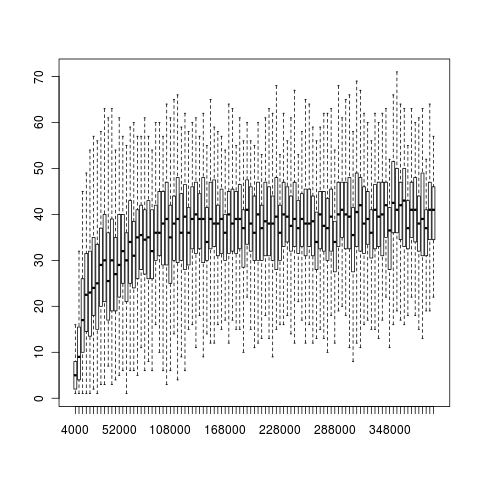
\includegraphics[height=4cm]{images/trajLimitedTanhAlive.png}
% %  \includegraphics[height=4cm]{images/trajLimitedTanhHistEnerg.png}
% %  \includegraphics[height=6cm]{images/trajLimitedTanhBarPlotEnergy.png}
% %  \end{figure}
% \end{itemize}

% 
\section{Experiments with no motion}
% The idea is to test wether or not medea is able to select "specialised" species, without other environmental constraints than the need to feed when two limited ressources are available.
% 
% In order to test that in a first time we are going to made robot unable to move, and to look how their habilities to forages 2 kinds of ressources evolve depending on how they are conncected, how genomes can spread, through the population.
% 
% Heatmap : we loose a bit of information : check gvalue for robots alive each n iteration : because robots are syncronized, we miss those who live less than a generation, who are 
\subsection{5 Environnements}
\newcommand{\imgSize}{0.45\textwidth}
% \begin{table}[ht]
% \caption{Five static environments}
% \centering
% \begin{tabular}{lcc}
% &Both ressources reachable &One ressource reachable \\
% \newline
% all linked&\includegraphics[width=\imgSize]{images/environments/staticEnv0}&\\
% \newline
% 2 groups,1 link&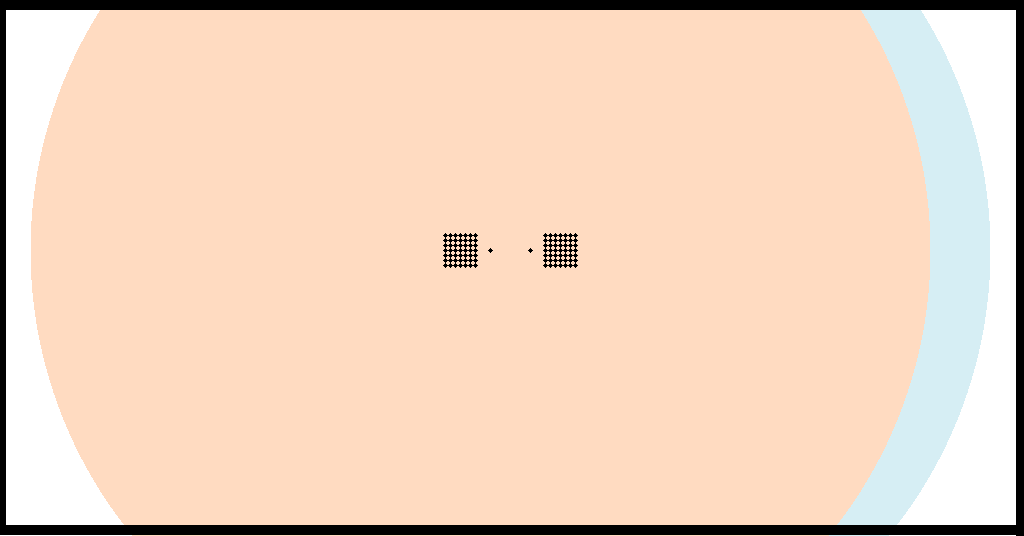
\includegraphics[width=\imgSize]{images/environments/staticEnv3}&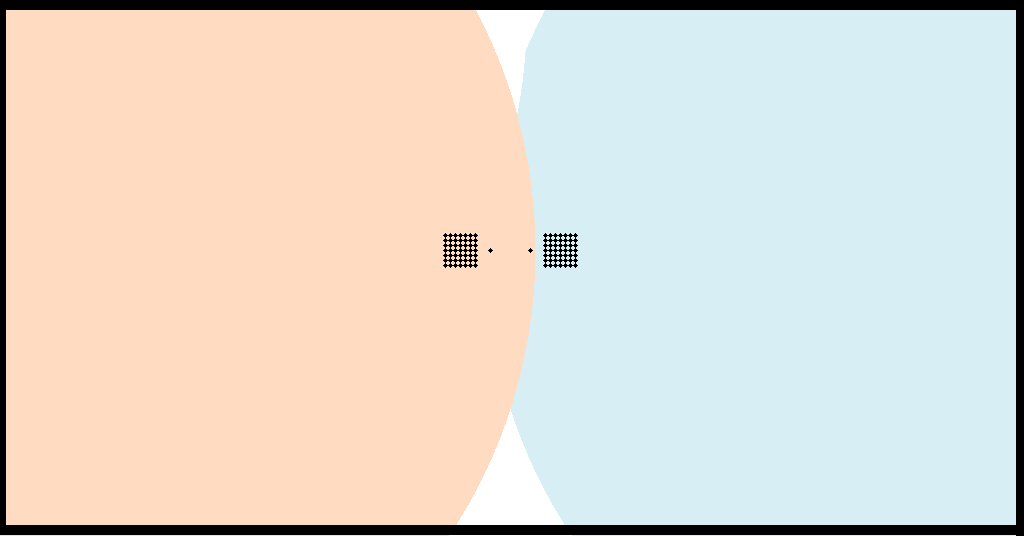
\includegraphics[width=\imgSize]{images/environments/staticEnv4}\\
% \newline
% Chain&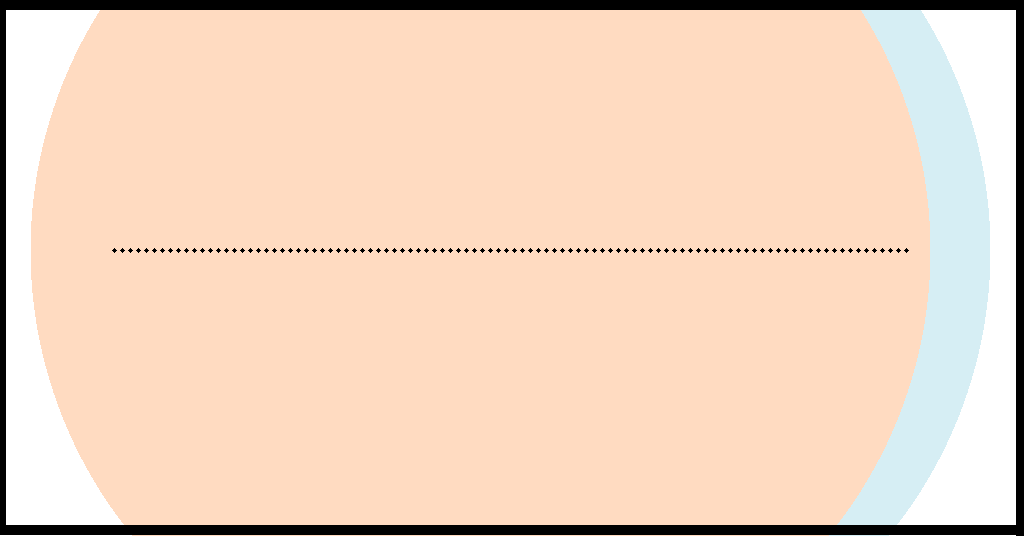
\includegraphics[width=\imgSize]{images/environments/staticEnv1}&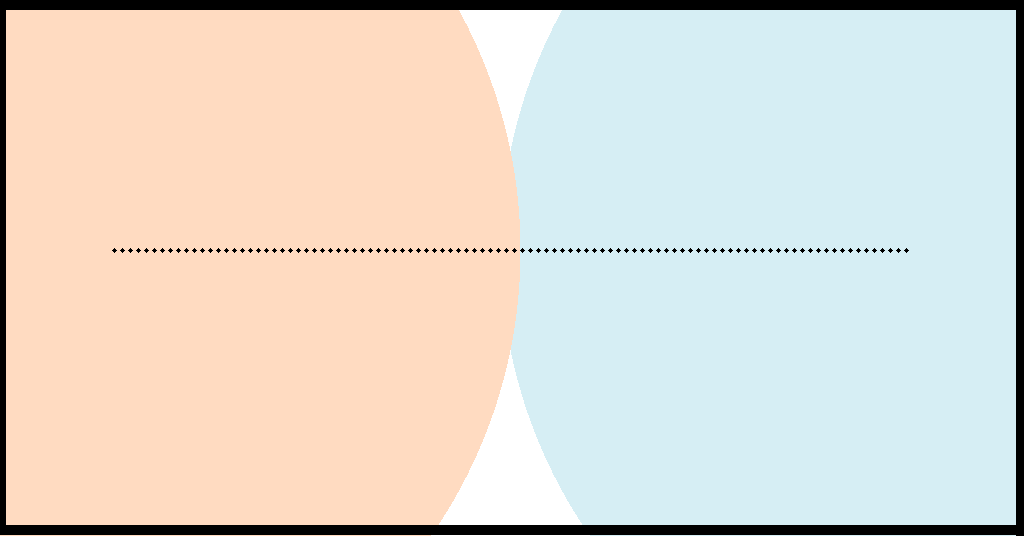
\includegraphics[width=\imgSize]{images/environments/staticEnv2}\\
% \end{tabular}
% \label{tab:gt}
% 
% \end{table}%
% All run have been done for 40\,000 iterations, with energyMax =1, 

\subsubsection{Static environment 0}
% All robots are on the same place, can exchanges their genome and use both ressources.
% Even here it works pretty well :

\begin{table}[h!]
 \caption{results for env0. \newline 
 The top right graph show number of active robots during a 150\,000 iteration's run with ressource availability at 50/50. As we can see if we wait a long time we will oscillate beetwen the two specialised populations. 
 \newline The two middle graphs illustrate the same thing : the ratio beetwen the number of individu foraging R1 and the ration of individu which exploit R2 at the end of a run. And this for all different ressource repartitions .
 \newline The two bottom graphs show the mean number (left graph) and the median(right graph) of active agents using R1 (dark grey) and r2 (light grey) respectively.}
 \centering
 \begin{tabular}{cc}
 \includegraphics[width=\imgSize]{images/5StaticEnv/environments/staticEnv0}&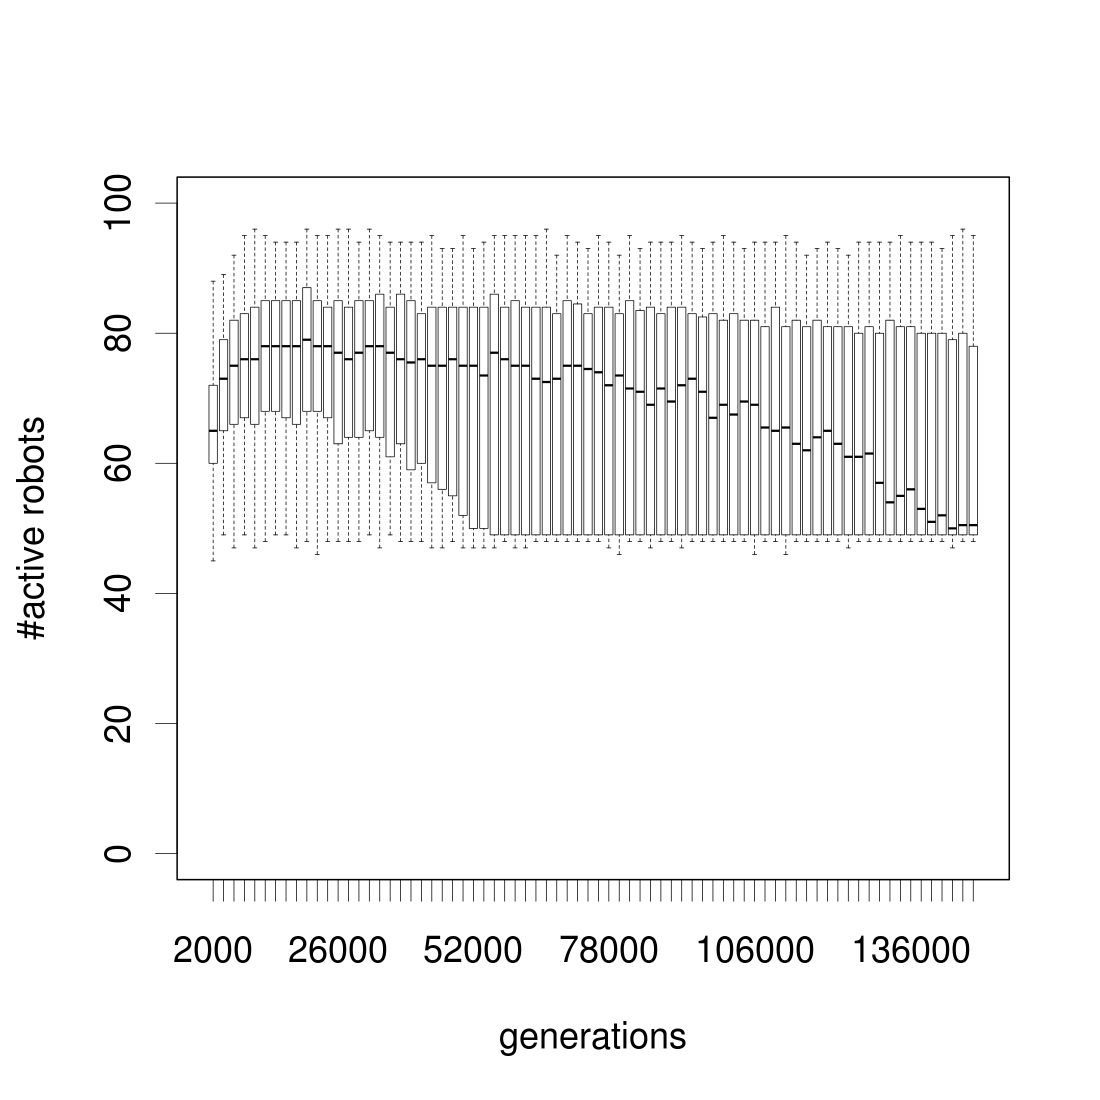
\includegraphics[width=\imgSize]{images/5StaticEnv/alive_staticEnv0}\\
 \newline
 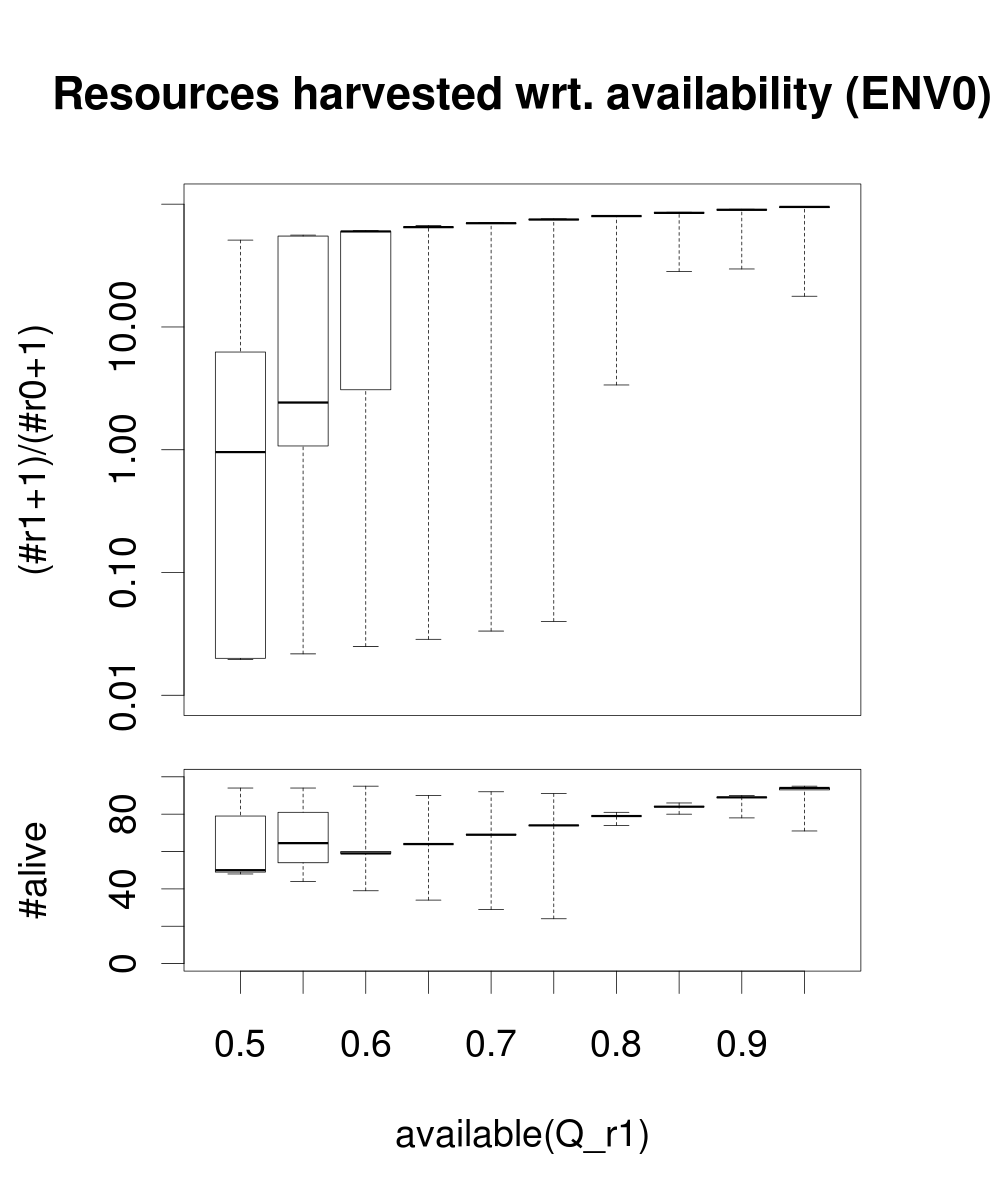
\includegraphics[width=\imgSize]{images/5StaticEnv/ratioAndRep_staticEnv0LogY}& 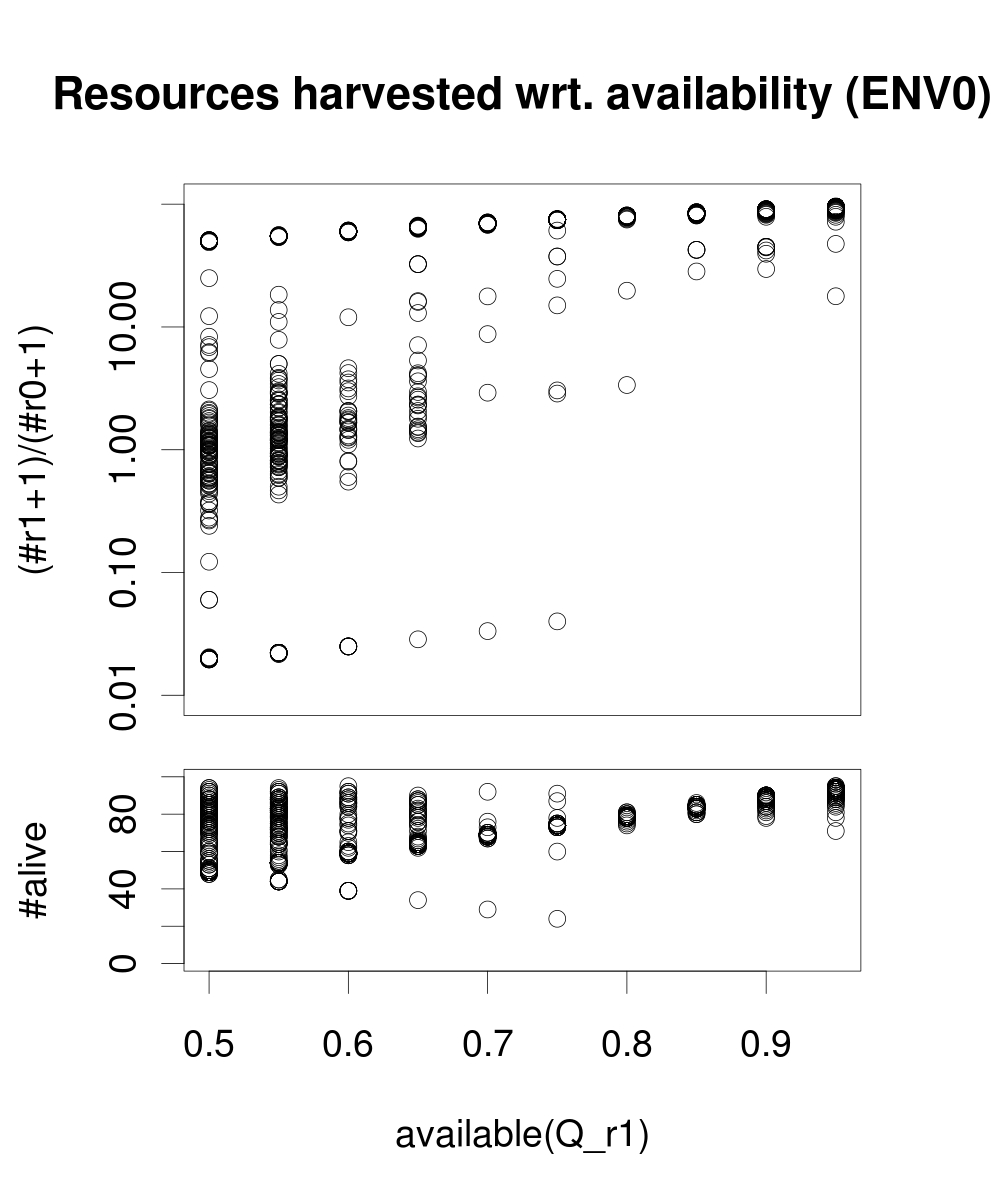
\includegraphics[width=\imgSize]{images/5StaticEnv/ratioAndRep_staticEnvPlot0LogY}\\
 \newline
 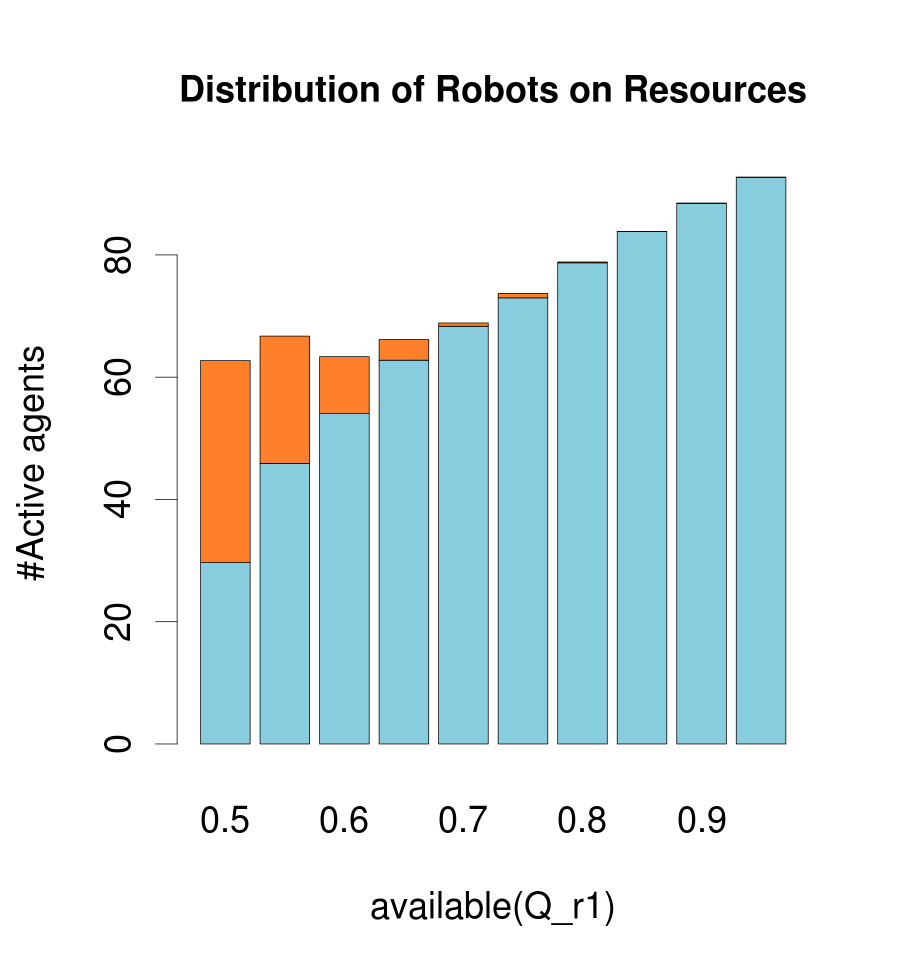
\includegraphics[width=\imgSize]{images/5StaticEnv/barplotAliveR1AndR2_mean_env0}& 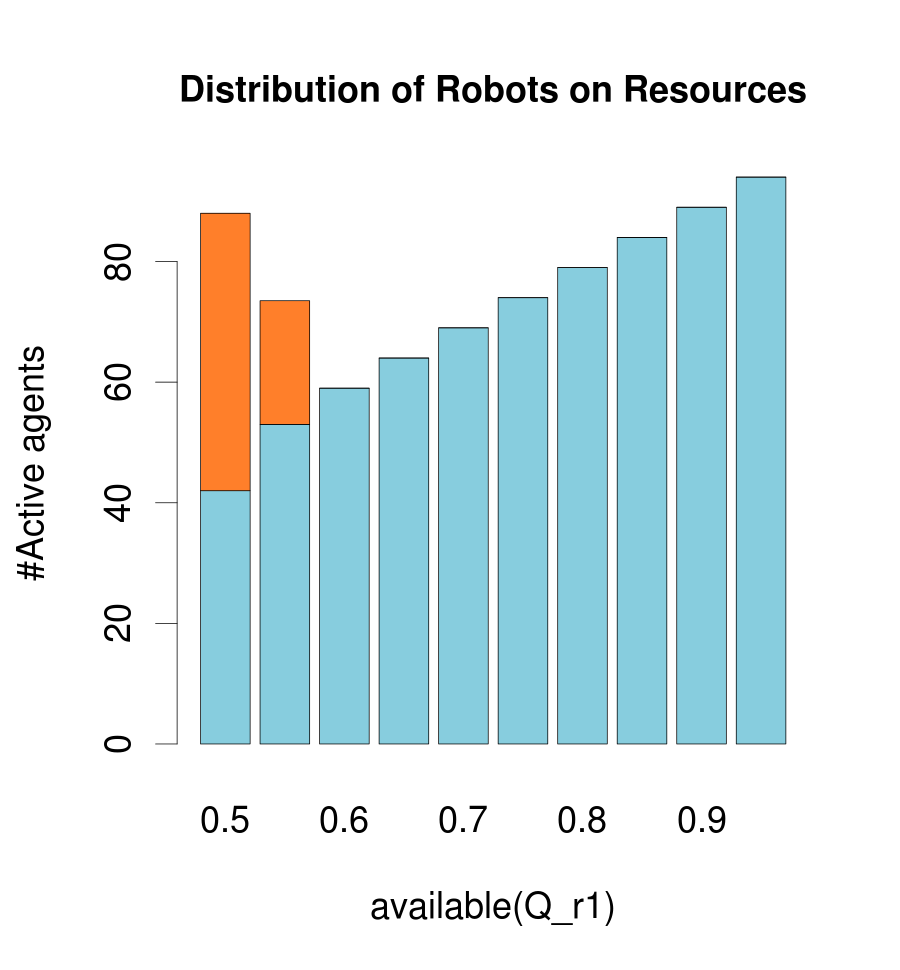
\includegraphics[width=\imgSize]{images/5StaticEnv/barplotAliveR1AndR2_median_env0}\\
 \end{tabular}
\end{table}
% \vspace{-1cm}
\begin{table}[h!]
\caption{Environment 0, Samples:\\On the left : the repartition of $g_{skill}$ in the whole population during the time ; on the right : the value of $g_{skill}$ for all robot during the time.\\ {\scriptsize \textbf{warnings : those graph show varitions of $g_{skill}$ during 150\,000 iterations for env0 but only during 40\,000 for the over environments} }}
\centering
\begin{tabular}{cc}
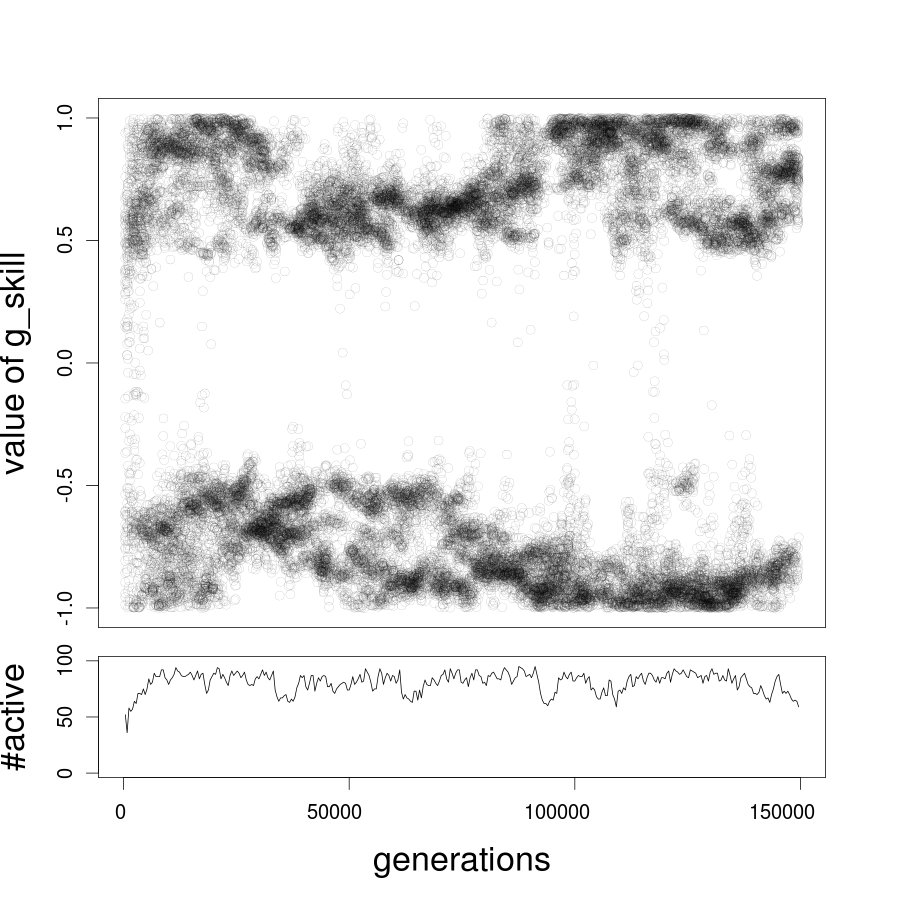
\includegraphics[width=\imgSize]{images/5StaticEnv/Gplot59_staticEnv0}&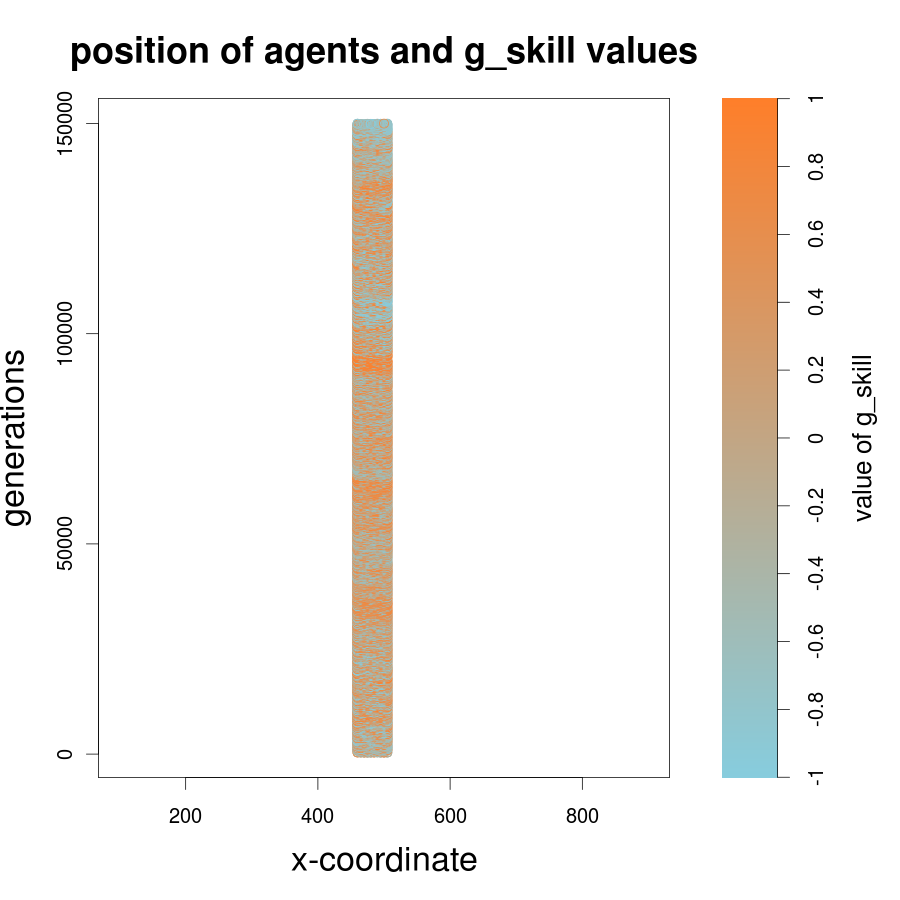
\includegraphics[width=\imgSize]{images/5StaticEnv/Gplot59Static_staticEnv0}\\
\newline
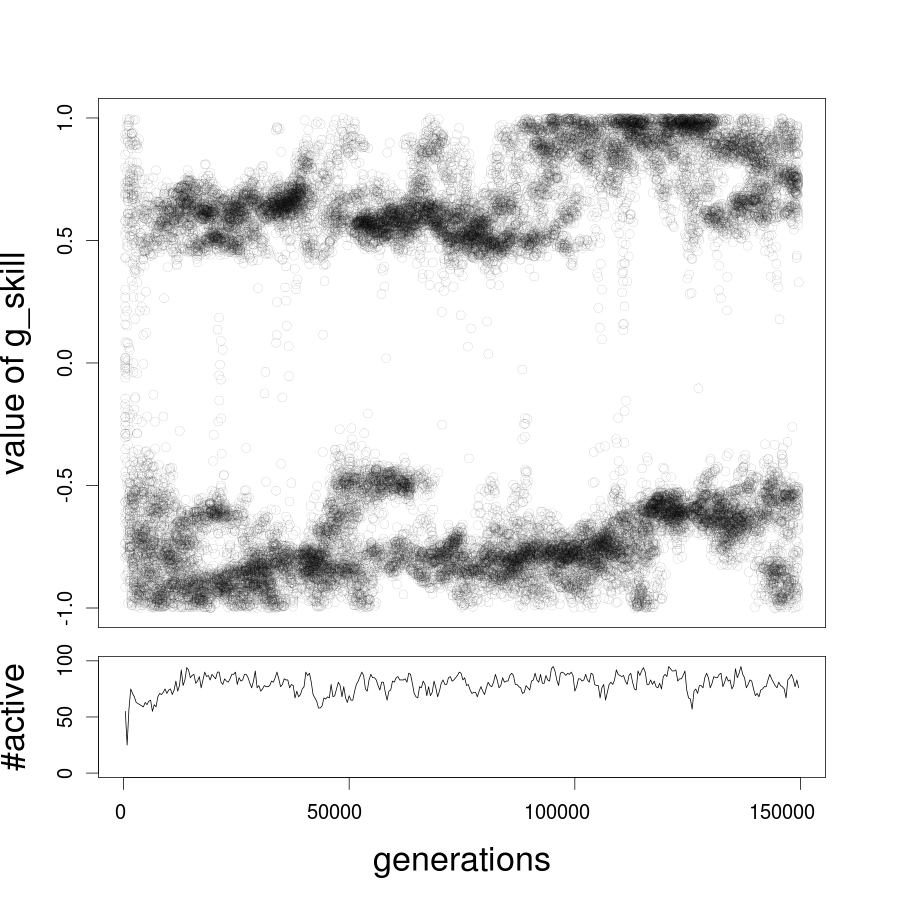
\includegraphics[width=\imgSize]{images/5StaticEnv/Gplot47_staticEnv0}&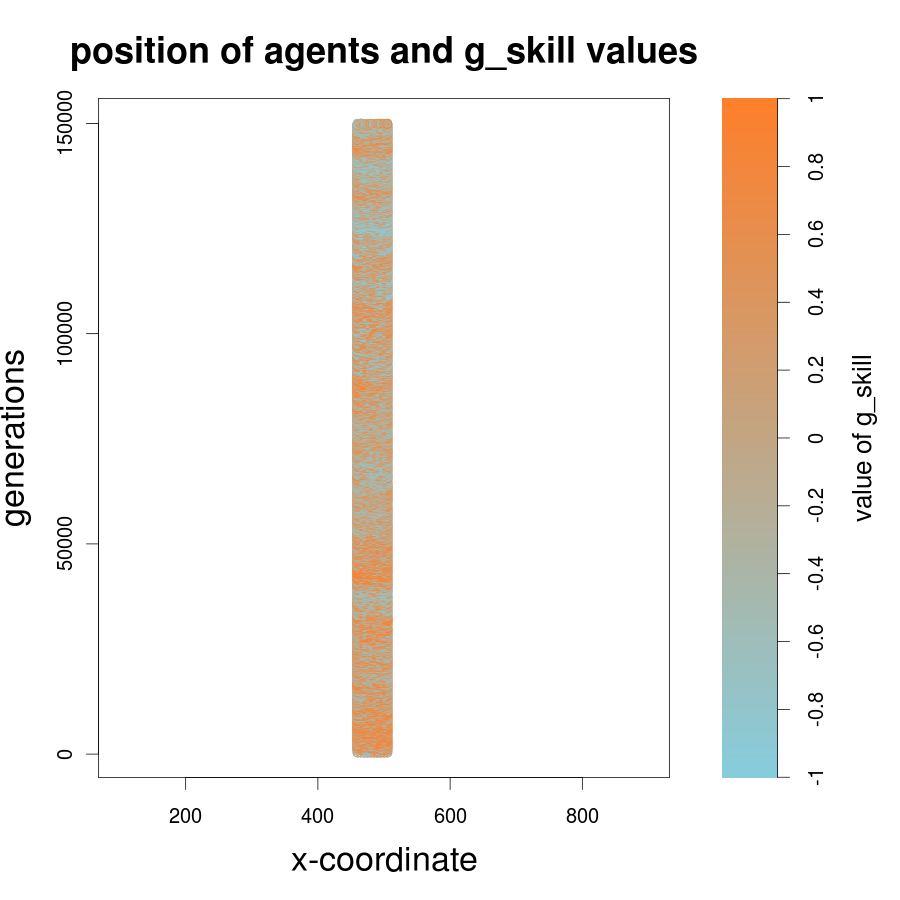
\includegraphics[width=\imgSize]{images/5StaticEnv/Gplot47Static_staticEnv0}\\
\newline
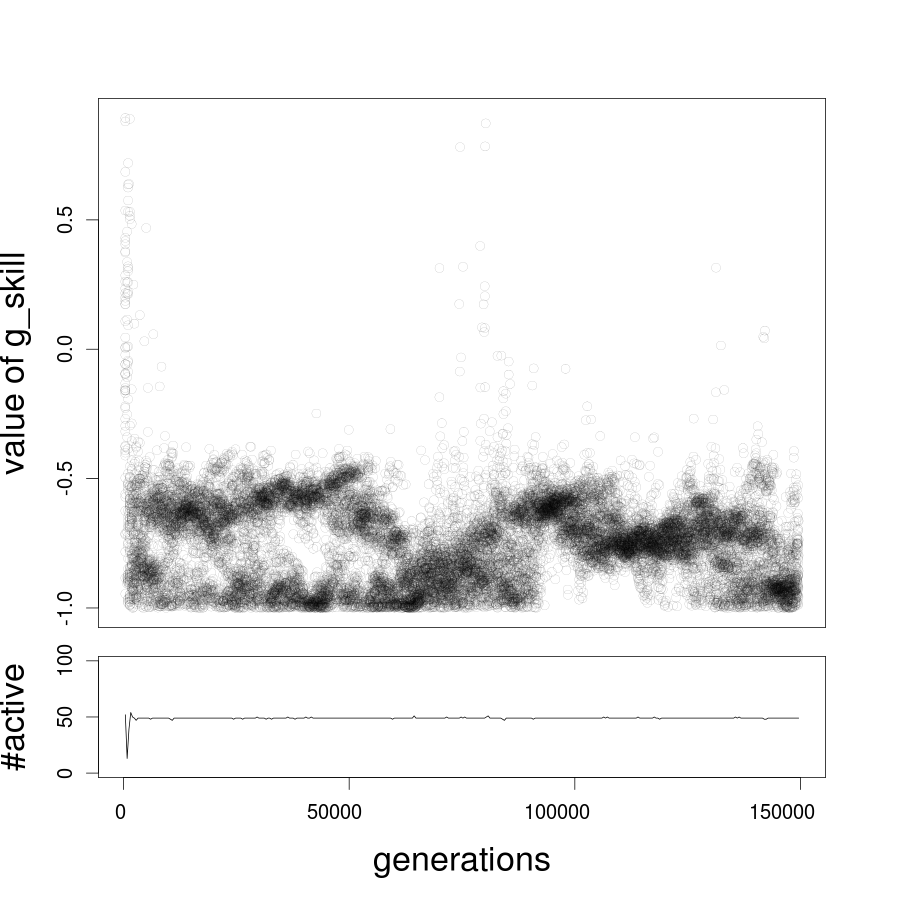
\includegraphics[width=\imgSize]{images/5StaticEnv/Gplot62_staticEnv0}&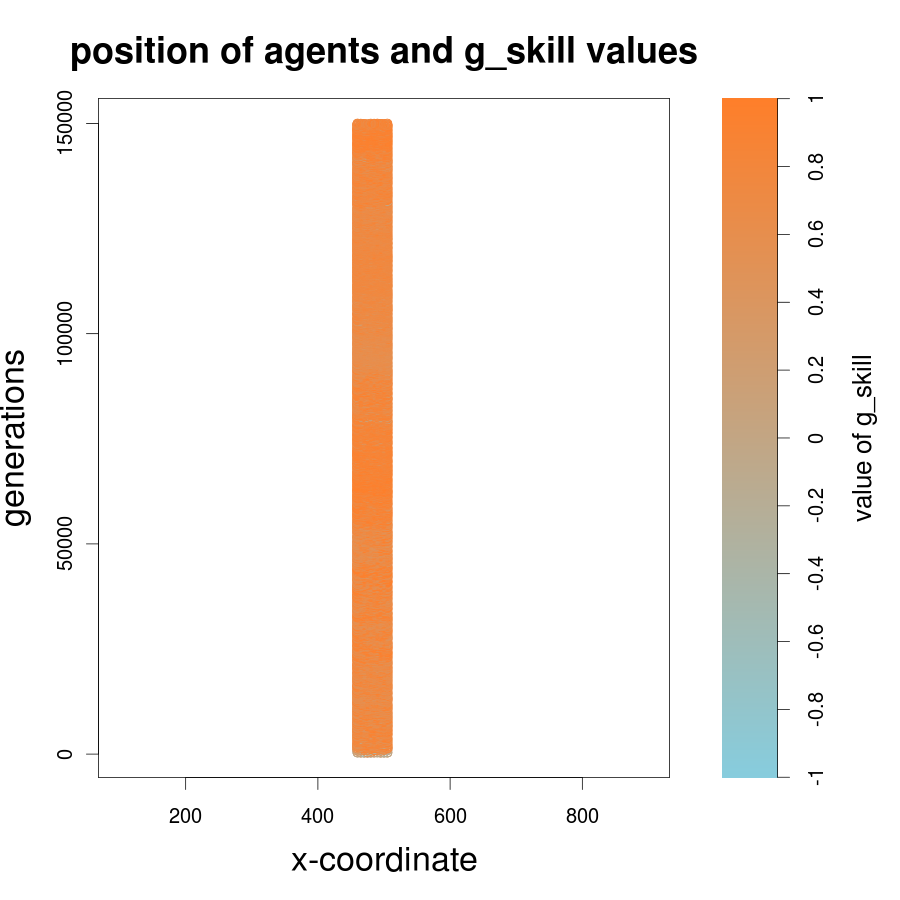
\includegraphics[width=\imgSize]{images/5StaticEnv/Gplot62Static_staticEnv0}\\
\newline
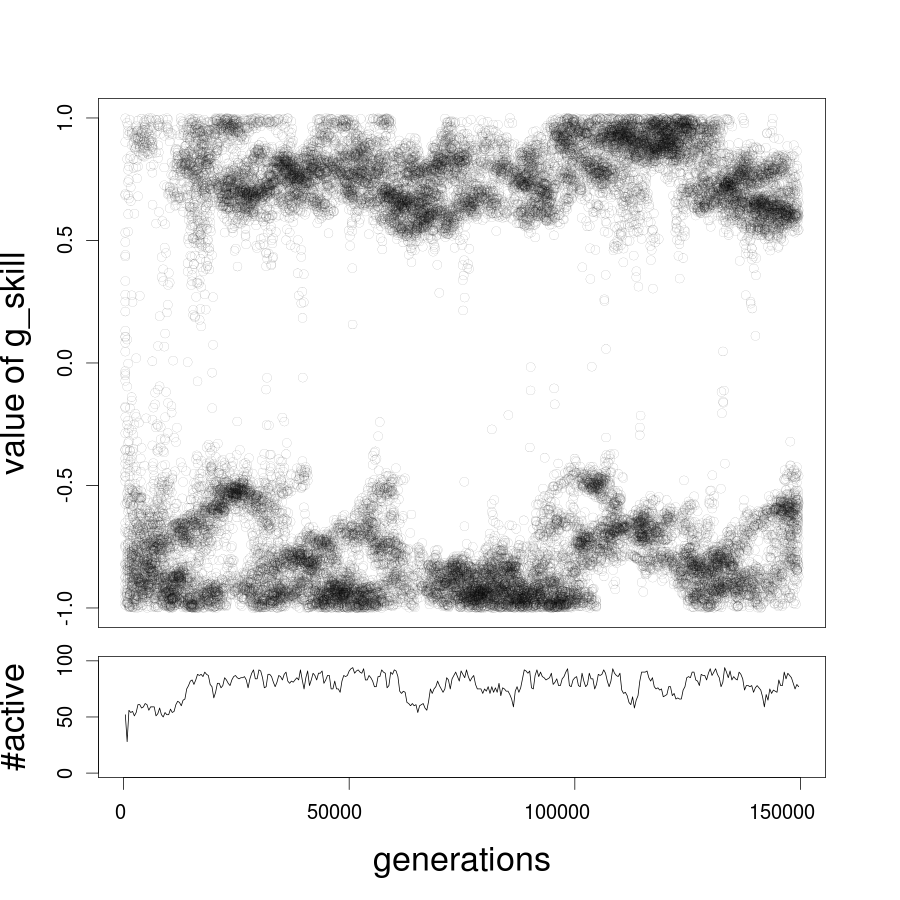
\includegraphics[width=\imgSize]{images/5StaticEnv/Gplot58_staticEnv0}&\includegraphics[width=\imgSize]{images/5StaticEnv/Gplot58Static_staticEnv0}\\
\end{tabular}

\end{table}

\subsubsection{Static environment 1}
\begin{table}[h!]
 \caption{results for env1.\newline On the bottom left graph we see that it is more diffult to maintain the theoritical ratio when the smallest subpopulation cannot be larger than 20 percent of the population. After that the biggest population overcome the environment. }
 \centering
 \begin{tabular}{cc}
 \includegraphics[width=\imgSize]{images/5StaticEnv/environments/staticEnv1}&\includegraphics[width=\imgSize]{images/5StaticEnv/alive_staticEnv1}\\
\newline
\includegraphics[width=\imgSize]{images/5StaticEnv/ratioAndRep_staticEnv1LogY}&\includegraphics[width=\imgSize]{images/5StaticEnv/ratioAndRep_staticEnvPlot1LogY}\\
 \newline
 \includegraphics[width=\imgSize]{images/5StaticEnv/barplotAliveR1AndR2_mean_env1}& \includegraphics[width=\imgSize]{images/5StaticEnv/barplotAliveR1AndR2_median_env1}
\end{tabular}
\end{table}

\begin{table}[h!]
\caption{Environment 1, Samples}
 \centering
 \begin{tabular}{cc}
 \includegraphics[width=\imgSize]{images/5StaticEnv/Gplot47_staticEnv1}&\includegraphics[width=\imgSize]{images/5StaticEnv/Gplot47Static_staticEnv1}\\
 \newline
 \includegraphics[width=\imgSize]{images/5StaticEnv/Gplot66_staticEnv1}&\includegraphics[width=\imgSize]{images/5StaticEnv/Gplot66Static_staticEnv1}\\
 \newline
 \includegraphics[width=\imgSize]{images/5StaticEnv/Gplot29_staticEnv1}&\includegraphics[width=\imgSize]{images/5StaticEnv/Gplot29Static_staticEnv1}\\
 \newline
 \includegraphics[width=\imgSize]{images/5StaticEnv/Gplot9_staticEnv1}&\includegraphics[width=\imgSize]{images/5StaticEnv/Gplot9Static_staticEnv1}\\
 \end{tabular}

\end{table}


\subsubsection{Static environment 2}
\begin{table}[ht]
\caption{results for env2}
\centering
\begin{tabular}{cc}
\includegraphics[width=\imgSize]{images/5StaticEnv/environments/staticEnv2}&\includegraphics[width=\imgSize]{images/5StaticEnv/alive_staticEnv2}\\
\newline
\includegraphics[width=\imgSize]{images/5StaticEnv/ratioAndRep_staticEnv2LogY}&\includegraphics[width=\imgSize]{images/5StaticEnv/ratioAndRep_staticEnvPlot2LogY}\\
 \newline
 \includegraphics[width=\imgSize]{images/5StaticEnv/barplotAliveR1AndR2_mean_env2}& \includegraphics[width=\imgSize]{images/5StaticEnv/barplotAliveR1AndR2_median_env2}
\end{tabular}
\end{table}

\begin{table}[ht]
\caption{Environment 2, Samples:
	\\The envirnomental setup (the reward function) does not allow a group to switch in a other one ; maybe the fitness gap beetwen the two phenotype is to wide.
}
 \centering
 \begin{tabular}{cc}
 \includegraphics[width=\imgSize]{images/5StaticEnv/Gplot22_staticEnv2}&\includegraphics[width=\imgSize]{images/5StaticEnv/Gplot22Static_staticEnv2}\\
 \newline
 \includegraphics[width=\imgSize]{images/5StaticEnv/Gplot66_staticEnv2}&\includegraphics[width=\imgSize]{images/5StaticEnv/Gplot66Static_staticEnv2}\\
 \newline
 \includegraphics[width=\imgSize]{images/5StaticEnv/Gplot5_staticEnv2}&\includegraphics[width=\imgSize]{images/5StaticEnv/Gplot5Static_staticEnv2}\\
 \newline
 \includegraphics[width=\imgSize]{images/5StaticEnv/Gplot92_staticEnv2}&\includegraphics[width=\imgSize]{images/5StaticEnv/Gplot92Static_staticEnv2}\\
 \end{tabular}

\end{table}

\subsubsection{Static environment 3}
\begin{table}[h!]
\caption{results for env3}
\centering
\begin{tabular}{cc}
\includegraphics[width=\imgSize]{images/5StaticEnv/environments/staticEnv3}&\includegraphics[width=\imgSize]{images/5StaticEnv/alive_staticEnv3}\\
\newline
\includegraphics[width=\imgSize]{images/5StaticEnv/ratioAndRep_staticEnv3LogY}&\includegraphics[width=\imgSize]{images/5StaticEnv/ratioAndRep_staticEnvPlot3LogY}\\
 \newline
 \includegraphics[width=\imgSize]{images/5StaticEnv/barplotAliveR1AndR2_mean_env3}& \includegraphics[width=\imgSize]{images/5StaticEnv/barplotAliveR1AndR2_median_env3}
\end{tabular}

\end{table}

\begin{table}[h!]
\caption{Environment 3, Samples}
 \centering
 \begin{tabular}{cc}
 \includegraphics[width=\imgSize]{images/5StaticEnv/Gplot5_staticEnv3}&\includegraphics[width=\imgSize]{images/5StaticEnv/Gplot5Static_staticEnv3}\\
 \newline
 \includegraphics[width=\imgSize]{images/5StaticEnv/Gplot8_staticEnv3}&\includegraphics[width=\imgSize]{images/5StaticEnv/Gplot8Static_staticEnv3}\\
 \newline
 \includegraphics[width=\imgSize]{images/5StaticEnv/Gplot51_staticEnv3}&\includegraphics[width=\imgSize]{images/5StaticEnv/Gplot51Static_staticEnv3}\\
 \newline
 \includegraphics[width=\imgSize]{images/5StaticEnv/Gplot99_staticEnv3}&\includegraphics[width=\imgSize]{images/5StaticEnv/Gplot99Static_staticEnv3}\\
 \end{tabular}

\end{table}

\subsubsection{Static environment 4}

\begin{table}[h!]
\caption{results for env4}
\centering
\begin{tabular}{cc}
\includegraphics[width=\imgSize]{images/5StaticEnv/environments/staticEnv4}&\includegraphics[width=\imgSize]{images/5StaticEnv/alive_staticEnv4}\\
\newline
\includegraphics[width=\imgSize]{images/5StaticEnv/ratioAndRep_staticEnv4LogY}&\includegraphics[width=\imgSize]{images/5StaticEnv/ratioAndRep_staticEnvPlot4LogY}\\
 \newline
 \includegraphics[width=\imgSize]{images/5StaticEnv/barplotAliveR1AndR2_mean_env4}& \includegraphics[width=\imgSize]{images/5StaticEnv/barplotAliveR1AndR2_median_env4}
\end{tabular}
\end{table}
\begin{table}[h!]
\caption{Environment 4, Samples}
 \centering
 \begin{tabular}{cc}
 \includegraphics[width=\imgSize]{images/5StaticEnv/Gplot17_staticEnv4}&\includegraphics[width=\imgSize]{images/5StaticEnv/Gplot17Static_staticEnv4}\\
 \newline
 \includegraphics[width=\imgSize]{images/5StaticEnv/Gplot40_staticEnv4}&\includegraphics[width=\imgSize]{images/5StaticEnv/Gplot40Static_staticEnv4}\\
 \newline
 \includegraphics[width=\imgSize]{images/5StaticEnv/Gplot62_staticEnv4}&\includegraphics[width=\imgSize]{images/5StaticEnv/Gplot62Static_staticEnv4}\\
 \newline
 \includegraphics[width=\imgSize]{images/5StaticEnv/Gplot58_staticEnv4}&\includegraphics[width=\imgSize]{images/5StaticEnv/Gplot58Static_staticEnv4}\\
 \end{tabular}

\end{table}

\begin{table}[ht]
 \centering
 \caption{À gauche les moyennes des rapports (les écarts types sont trops importants, sachant que parfois le rapport est assez faible : il y a deux sous populations ; parfois il est proche de 100 : il n'y a qu'une population, ce qui brouille beaucoup le graphe), à droite les rapports théoriques si les deux populations étaient réparties parfaitement pour utiliser l'environnement au mieux. On voit que là où les deux ressources sont accessible simultanéments (env0, 1 et 3), plus les idindivuds sont connectés (env0 et env3) plus il est difficile de maintenir un ratio proche du ratio théorique.}
 \begin{tabular}{cc}
 \includegraphics[width=\imgSize]{images/5StaticEnv/ratioR1R2foreachEnv}&\includegraphics[width=\imgSize]{images/5StaticEnv/theroticalRatios.png}\\
 \newline
 \end{tabular}
\end{table}

% \subsection{Summary for all env without penality:}
% \begin{table}
%  \begin{tabular}{ | r | c c c c c |} 
% \hline
%  & 0 & 1 & 2 & 3 & 4\\
% \hline
% mean & 24.93959 & 5.963317 & 2.889211 & 22.96007 & 2.887429\\
% sd & 41.18270 & 20.044163 & 9.577123 & 40.42920 & 9.286529\\
% \hline
% \end{tabular}
% \caption{Ratio $\frac{\#R1+1}{\#R2+1}$ for the 5th different environments without pressure}
% \end{table}
\end{document}




% \subsection{Summary for all env without penality:}
% \begin{table}
%  \begin{tabular}{ | r | c c c c c |} 
% \hline
%  & 0 & 1 & 2 & 3 & 4\\
% \hline
% mean & 24.93959 & 5.963317 & 2.889211 & 22.96007 & 2.887429\\
% sd & 41.18270 & 20.044163 & 9.577123 & 40.42920 & 9.286529\\
% \hline
% \end{tabular}
% \caption{Ratio $\frac{\#R1+1}{\#R2+1}$ for the 5th different environments without pressure}
% \end{table}
\end{document}

#suppress extections runs

dataPropre=supprExtinction(data,length=800000)
data_activePropre=supprExtinction(data_active,length=800000)
data_energyPropre=supprExtinction(data_energy,length=800000)

#get extracted Dataz
data=read.csv("logs_genometracking.csv")
# data_energy=read.csv("logs_ancestors.csv")
data_active=read.csv("logs_actives.csv")
source("~/evorob/Dev/Roborobo/perso/simon/lineage/Rscript/plotg.R")

drawAllGraph(supprExtinction(data,length=300000),supprExtinction(data_active,length=300000))

png("~/evorob/Perso/Simon/doc/images/env-8l_rew-t_res-l_mat_tax-1MhBarPlotEnergy.png")
barplotEnergy(data_energy)
dev.off()
png("~/evorob/Perso/Simon/doc/images/env-8l_rew-t_res-l_mat_tax-1MhHistEnerg.png")
hist(data$Iteration[data_energy$r0 > 0 & data_energy$r1 >0],nclass=max(data_energy$Iteration)/10000,lwd=2)
dev.off()
plot(data$At, data$Iteration,col=ramp[as.integer(500*(data$GValue+1))+1],lwd=2)

rm complete*  logs/* && cp ../roborobo .
##############
png("~/evorob/Perso/Simon/doc/images/alive_staticEnv4.png")
plotActive(data_active,res=400,lwd=1,ylim=c(0,100),xlim=c(0,80))
dev.off()

png("~/evorob/Perso/Simon/doc/images/Gplot1Static_staticEnv2.png")
plotGFixedPos(data[data$Sim == 0,])
dev.off()

png("~/evorob/Perso/Simon/doc/images/Gplot1_staticEnv2.png")
plotGandReward(data[data$Sim == 0,],data_active[data_active$Sim == 0,],lwd=1,col=F)
dev.off()


mkdir logs
mv *.txt logs
/home/simon/evorob/Dev/Roborobo/perso/simon/lineage/followaGene.sh 1 10000000 logs 1 > result.csv

cd simon/Roborobo/
vim config/medea-sp.properties
perso/jeanmarc/grid5000/runParallal.sh 100 config/medea-sp.properties 8

scp -r logs/ scarrignon@frontend:~/logs_$HOSTNAME 

rm lastRunDone complete112509631813981 logs/*
perso/jeanmarc/grid5000/runParallal.sh 100 config/medea-sp.properties 8





 png("~/evorob/Perso/Simon/doc/images/Gplot58Static_staticEnv0.png")
 plotGFixedPos(data[data$Sim == 58,])
 dev.off()
 png("~/evorob/Perso/Simon/doc/images/Gplot58_staticEnv0.png")
 plotGandReward(data[data$Sim == 58,],data_active[data_active$Sim == 58,],col=F)
 dev.off()
 png("~/evorob/Perso/Simon/doc/images/Gplot62Static_staticEnv0.png")
 plotGFixedPos(data[data$Sim == 62,])
 dev.off()
 png("~/evorob/Perso/Simon/doc/images/Gplot62_staticEnv0.png")
 plotGandReward(data[data$Sim == 62,],data_active[data_active$Sim == 62,],col=F)
 dev.off()
plotGandReward(data[data$Sim == 47,],data_active[data_active$Sim == 47,],col=F)
 dev.off()
 png("~/evorob/Perso/Simon/doc/images/Gplot47Static_staticEnv0.png")
 plotGFixedPos(data[data$Sim == 47,])
 dev.off()
 png("~/evorob/Perso/Simon/doc/images/Gplot47_staticEnv0.png")
 plotGandReward(data[data$Sim == 47,],data_active[data_active$Sim == 47,],col=F)
 dev.off()
 png("~/evorob/Perso/Simon/doc/images/Gplot59Static_staticEnv0.png")
 plotGFixedPos(data[data$Sim == 59,])
 dev.off()
 png("~/evorob/Perso/Simon/doc/images/Gplot59_staticEnv0.png")
 plotGandReward(data[data$Sim == 59,],data_active[data_active$Sim == 59,],col=F)
 dev.off()



